\section{Introduction}

\begin{figure}[t]
\centering
\includegraphics[width=0.45\textwidth]{figures/taxonomylabels}
 \caption{An example of geographical taxonomy with labels}
\label{fig:toytaxonomyexample}
\end{figure}


A string join, which finds all equivalent string pairs between two input collections, is an essential operation in many applications, such as  data integration \cite{conf/sigmod/Sarawagi04}, data cleansing \cite{conf/vldb/ArasuGK06,journals/www/LiJM06} and record linkage \cite{books/Winkler99}. In practice, the same object/entity may have different representations  due to a variety of reasons such as misspellings
caused by typographic errors and different formatting conventions including synonyms, abbreviations and acronyms. Hence, it is important to support approximate string joins for reconciling different
representations of an entity. A large number of  similarity functions such as Levenshtein distance~\cite{conf/sigmod/WangLF12},
Hamming distance~\cite{conf/spire/Kondrak05}, Episode
distance~\cite{conf/ijcai/CohenRF03}, Cosine
metric~\cite{journals/ipm/SaltonB88}, Jaccard
Coefficient~\cite{conf/icde/ChaudhuriGK06,conf/icde/LiLL08}, JaccT \cite{conf/icde/ArasuCK08} and Synonym-based similarity \cite{conf/sigmod/LuLWLW13} have been proposed in the literature. It is well known
that no single similarity function is universally applicable
across all domains and scenarios.

In this paper, we investigate a novel problem to exploit taxonomy with string similarity joins. In principle, the taxonomy presents a general purpose strategy to improve the accuracy of string joins by enriching data with semantics-based knowledge. Taxonomies are sets of IS-A hierarchies, which identify the relations between different concepts. The IS-A relationship
is a transitive closure of the concept-instance relationship.
For example, if ``\textsf{kitten}'' is an instance of ``\textsf{cat}'', and
``\textsf{cat}'' is an instance of ``\textsf{pet}'', then ``\textsf{kitten}'' is an instance
of ``\textsf{pet}''. If we treat each term as a node, and create
for each (concept, instance) pair, an edge from the concept
to the instance, then we can think of the taxonomy as a tree or forest. For any node that representing a term,
the IS-A relation could be any descendant of it in the tree. Figure
\ref{fig:toytaxonomyexample} gives a toy example of a geographical taxonomy tree.

Based on the taxonomy,  the similarity of two strings can be measured in a \textit{semantic} way. For example, consider two pairs (\textsf{Los Angles}, \textsf{Cupertino}) and (\textsf{Los Angles}, \textsf{Seoul}). Intuitively, the similarity between \textsf{Los Angles} and \textsf{Cupertino} should be greater than that between \textsf{Los Angles} and \textsf{Seoul}, because the formers are two cities in the same country and the same state. To quantify the similarity, one method is to calculate the longest common prefixes (LCP) between two strings against the taxonomy. Thus, based on Figure \ref{fig:toytaxonomyexample}, LCP(\textsf{Los Angles}, \textsf{Cupertino})= 4, but (\textsf{Los Angles}, \textsf{Seoul})=1. Clearly the similarity between \textsf{Los Angles} and \textsf{Cupertino} is greater than that between \textsf{Los Angles} and \textsf{Seoul}.


\begin{figure}[t]
\centering
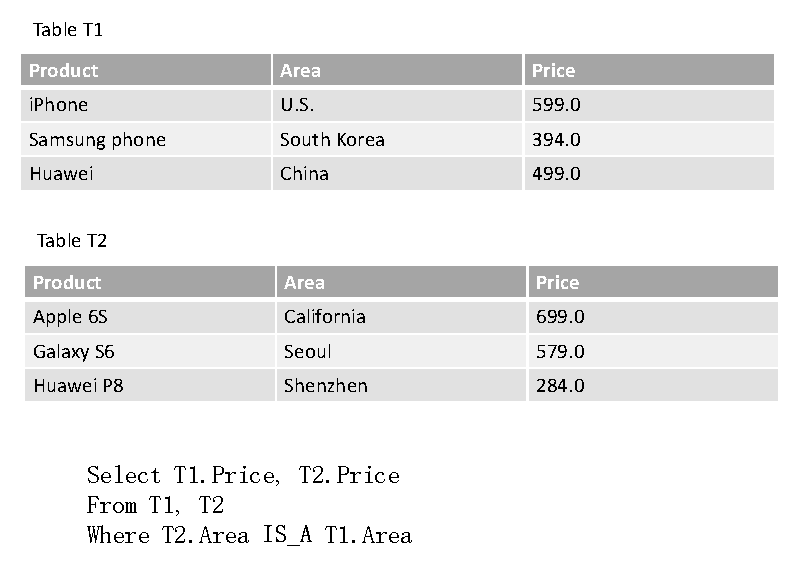
\includegraphics[width=0.45\textwidth]{figures/productexample}
 \caption{Two tables for data integration}
\label{fig:twotables}
\end{figure}

We give several applications to shed light on the importance of the  string similarity matching with taxonomy on databases.

\begin{itemize}
  \item \textbf{Data Integration} ~ Data integration involves combining data residing in different sources. Taxonomy is quite useful to  discover the relations of various objects. For example, consider two tables in Figure \ref{fig:twotables}. In order to correctly perform the integration between two tables, the system needs to know hat ``\textsf{Apple 6s is a model of iphone}'' and ``\textsf{Cupertino is a city in US}'', and etc. A join mechanism that can utilize such taxonomy knowledge may help users to discover more relevant records and thus to improve the effectiveness of data integration.
  \item \textbf{Data mining} ~ Term classification and term clustering are two important tasks in data mining. A new similarity measure that can find the IS-A relations between terms is beneficial to term classification and clustering algorithms to improve their accuracies \cite{journals/dke/CaglieroG13}.
  \item \textbf{Data cleaning}~  Data cleaning is the process of detecting and correcting (or removing) corrupt or inaccurate records from a table or database. Two records about ``\textsf{Sumsung cellphone}'' and ``\textsf{Glaxy S6}'' may contain the duplicate or inconsistent information, because ``\textsf{Glaxy S6}'' IS-A model of ``\textsf{Sumsung cellphones}''. In those scenarios, the taxonomy enhances the quality of data cleaning by finding more relevant records.

\end{itemize}

  %\item \textbf{Information extraction} Find all geological entity in U.S. Then a new similarity measure based on a geological taxonomy can handle term variation and discover more location of interests


%  Conceptually, there are two cases of string joins: \textit{exact-joins} and \textit{approximate-joins}. Exact joins mean that two matching strings are exactly the same, while approximate joins tolerate certain difference between two strings and the similarity between two strings is measured by a similarity function, such as  Levenshtein distance~\cite{conf/sigmod/WangLF12},
%Hamming distance~\cite{conf/spire/Kondrak05}, Episode
%distance~\cite{conf/ijcai/CohenRF03}, Cosine
%metric~\cite{journals/ipm/SaltonB88}, Jaccard
%Coefficient~\cite{conf/icde/ChaudhuriGK06,conf/icde/LiLL08}, and Dice
%similarity~\cite{conf/www/BayardoMS07}.



In this paper, we assume that we already have complete
information of these IS-A relations, i.e. \textit{taxonomy}, and we will focus on how
to efficiently perform a string join by utilizing the taxonomy, and how to optimize the index structure
for this purpose.

%For example, the (Guangdong, Shenzhen) is a (concept, instance) pair and (Shenzhen, China) has the IS-A relation, as Shenzhen is a city in China.


To support the string joins with taxonomy, the first step is to devise new similarity functions which can utilize the taxonomy. Although there is a wealth of research on string similarity functions, most of them focus only on the syntactical-level of words. Some emerging works  \cite{conf/icde/ArasuCK08} can utilize the synonyms to performs the string join, which use semantic information for word comparing. But their works cannot be easily extended to handle taxonomy, because  taxonomy represent a tree-like structure, which is more complicated than the binary relations as specified in synonyms (See Section 2 for more explanations of why the existing similarity functions are not applicable for taxonomy).



%\noindent which selects the prices of phones from two tables by performing the two IS-A joins against ``\textsf{product}'' and %``\textsf{area}'' columns (e.g. ``\textsf{Galaxy S6}'' is a model of ``\textsf{Samsung}'' in the \texttt{product} column and %``\textsf{Seoul}'' is a city of ``\textsf{South Korea}'' in the \texttt{area} column).

We first define the similarity between two nodes in the taxonomy, then we use the maximum weighted bipartite model to define the similarity of two strings.

Given the newly similarity functions TS and ETS, it is imperative to study efficient similarity join algorithms. The brute-force algorithm that enumerates every string pair and checks whether the two strings in the pair are similar is rather expensive. To alleviate this problem, many algorithms have been proposed in the recent two decades. One widely-adopted technique employs a filter-verification framework, which includes two steps: (1) Filter step: devising effective filtering algorithms to prune large numbers of dissimilar pairs and generating a set of candidate pairs; and (2) Verification step: verifying each candidate pair by computing
the real similarity and outputting the final results. Filtering algorithms in the first step play an important role
in the framework. Most of existing filtering algorithms employ a signature-based technique, which generates signatures for each string such that if two strings are similar, their signatures must have overlaps. Thus the signature-based technique can prune string pairs that have no common signature.

Recently many filtering techniques have been proposed, e.g., count filtering [8,13,18], length filtering [8,14], position
filtering [25,27], prefix filtering [4] and content filtering [25]. As prefix filtering is the most effective filtering technique,
many algorithms have been proposed to optimize prefix filtering for different similarity metrics, e.g., AllPair [2],
PPJoin [27], EDJoin [25], QChunk [17], VChunk [24], AdaptJoin [23]. There are also many other signature schemes, e.g., PartEnum [1],
PassJoin [14], FastSS [20].

Unfortunately, these algorithms are not easily extended to process taxonomy. Because all the existing methods are based on the observation that two strings are similar only if their signatures overlap. But this is not true for taxonomy, because two strings may have IS-A relation without any common tokens (signatures).

Our technical contribution here is to propose a new filtering strategy based on ETS similarity function. We first extend prefix scheme to propose n-ary prefix scheme. This n-ary prefix scheme has the independent interests in that it can outperform the state-of-art algorithms  for similarity joins even without the taxonomy. And then introduce the taxonomy node into the signature set and generate a composite signature scheme. We show that our n-ary prefix
filter has larger pruning power and less filtering cost
than state-of-the-art filters in a theoretical analysis based on Jaccard similarity.


Finally, we perform experiments to evaluate our results and show the benefits of proposal algorithms.

%\subsection{Novelty and contributions}
%
%Our contributions are as follows.
%\noindent \textbf{Introduction of taxonomy for string joins}. We introduce a new problem to utilize the taxonomy for the string joins in databases, which has application in data integration and data cleansing. We propose a novel
%
%\noindent \textbf{Optimal algorithms for TS} We develop an inverted list introduce an algorithm for multiple string joins.
%
%\noindent \textbf{Novel filters for ETS function} We extend TS to handle more general cases of strings with taxonomy and propose a composite n-ary signatures.
%
%\noindent \textbf{Generality and variations}  We introduce a novel algorithm for incrementally updating taxonomy. Our merging algorithm allows us to incorporate new correlations introduced over a subset of tuples into
%the correlations already present in the database, without recomputing the existing results.



\smallskip

The rest of this paper is organized as follows. Section 2
provides the necessary definitions, formulates . Section
3 includes our algorithm for exact joins with taxonomy. In Section 4, we study
the approximate string join, proposing our solution, analyzing its approximation
ratio, and presenting our similarity join algorithms.
Our experiments are presented in Section 5. Finally,
Section 6 concludes with a discussion about future work.
